
Our proof of the finishing lemma in Case B has the same structure as the finishing lemma in Case A, except we first construct the colour switchers in the ND-colouring in two steps, before showing this can be done with random vertices and colours. In overview, in this section we do the following, noting the lemmas in which the relevant result is given and the comparable lemmas in Section~\ref{sec:finishA}.
\begin{itemize}
\item Lemma~\ref{lem-switchpath}: We construct colour switchers in the ND-colouring for any pair of colours $(c_1,c_2)$ -- that is, two short rainbow paths with the same length between the same pair of vertices, whose colours are the same except that one uses $c_1$ and one uses $c_2$.
\item Lemma~\ref{lem-absorbpath}: We use Lemma~\ref{lem-switchpath} to construct a similar colour switcher in the ND-colouring that can use 1 of a set of 100 colours.
\item Lemma~\ref{lem-randabsorbpath}: We show that, given a pair of independent random vertex and colour sets, many of these switchers use only vertices and (non-switching) colours in the subsets (cf.\ Lemma~\ref{absorbA}).
\item Lemma~\ref{absorbBmacro}: We use distributive absorption to convert this into a larger scale absorption property (cf.\ Lemma~\ref{absorbAmacro}).
\item Lemma~\ref{colourcoverB}: We embed paths while ensuring that an (arbitrary) small set of colours is used (cf.\ Lemma~\ref{colourcover}).
\item Lemma~\ref{finishingB}: We embed paths using almost all of a set of colours, in such a way that this can reduce the number of `non-random' colours (cf.\ Lemma~\ref{Lemma_saturating_matching_lemma}).
\item Finally, we put this all together to prove Lemma~\ref{lem:finishB}, the finishing lemma in Case B (cf.\ the proof of Lemma~\ref{lem:finishA}).
\end{itemize}

\subsection{Colour switching with paths}\label{sec:switchers}
We start by constructing colour switchers in the ND-colouring capable of switching between 2 colours.
We use switchers consisting of two paths with length 7 between the same two vertices. By using one path or the other we can choose which of two colours $c_1$ and $c_2$ are used, as the other colours used appear on both paths.


\begin{defn}
In a complete graph $K_{2n+1}$ with vertex set $[2n+1]$, let $(x_0,a_1,\ldots,a_\ell)$ denote the path with length $\ell$ with vertices $x_0x_1\ldots x_\ell$ where, for each $i\in [\ell]$, $x_i=x_{i-1}+a_i\pmod 2n+1$.
\end{defn}


\begin{figure}[h]
\begin{center}
{
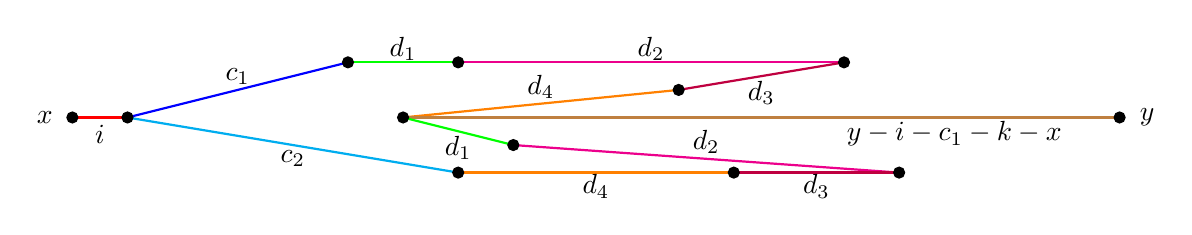
\begin{tikzpicture}[scale=0.7]
\draw [red,thick] (-1,0) -- (0,0);
\draw (-0.5,-0.3) node {$i$};
\draw [blue,thick] (4,1) -- (0,0);
\draw (2,0.75) node {$c_1$};
\draw [green,thick] (4,1) -- (6,1);
\draw (5,1.25) node {$d_1$};
\draw [magenta,thick] (13,1) -- (6,1);
\draw (9.5,1.25) node {$d_2$};
\draw [purple,thick] (13,1) -- (10,0.5);
\draw (11.5,0.45) node {$d_3$};
\draw [orange,thick] (5,0) -- (10,0.5);
\draw (7.5,0.55) node {$d_4$};
\draw [brown,thick] (5,0) -- (18,0);
\draw (15,-0.3) node {$y-i-c_1-k-x$};
\draw [green,thick] (5,0) -- (7,-0.5);
\draw (6,-0.55) node {$d_1$};
\draw [magenta,thick] (14,-1) -- (7,-0.5);
\draw (10.5,-0.45) node {$d_2$};
\draw [purple,thick] (14,-1) -- (11,-1);
\draw (12.5,-1.25) node {$d_3$};
\draw [orange,thick] (6,-1) -- (11,-1);
\draw (8.5,-1.25) node {$d_4$};
\draw [cyan,thick] (6,-1) -- (0,0);
\draw (3,-0.75) node {$c_2$};

\draw [fill=black] (-1,0) circle [radius = 0.1cm];
\draw [fill=black] (18,0) circle [radius = 0.1cm];
\draw [fill=black] (0,0) circle [radius = 0.1cm];
\draw [fill=black] (4,1) circle [radius = 0.1cm];
\draw [fill=black] (6,1) circle [radius = 0.1cm];
\draw [fill=black] (13,1) circle [radius = 0.1cm];
\draw [fill=black] (10,0.5) circle [radius = 0.1cm];
\draw [fill=black] (5,0) circle [radius = 0.1cm];
\draw [fill=black] (7,-0.5) circle [radius = 0.1cm];
\draw [fill=black] (6,-1) circle [radius = 0.1cm];
\draw [fill=black] (11,-1) circle [radius = 0.1cm];
\draw [fill=black] (14,-1) circle [radius = 0.1cm];

\draw (18.5,0) node {$y$};
\draw (-1.5,0) node {$x$};
\end{tikzpicture}
}
\end{center}
\caption{Two $x,y$-paths used to switch colours between $c_1$ and $c_2$.}\label{colourswitcher}
\end{figure}


\begin{lemma}[1 in 2 colour switchers]\label{lem-switchpath}
Let $1\gg n^{-1}$ and suppose that $K_{2n+1}$ is ND-coloured. Suppose we have a pair of distinct vertices $x,y\in V(K_{2n+1})$, a pair of distinct colours $c_1,c_2\in C(K_{2n+1})$, and sets $X\subset V(K_{2n+1})$ and $C\subset C(K_{2n+1})$ with $|X|\leq n/25$ and $|C|\leq n/25$.

Then, there is some set $C'\subset C(K_{2n+1})\setminus (C\cup\{c_1,c_2\})$ with size $6$ so that, for each $i\in \{1,2\}$, there is a $(C'\cup\{c_i\})$-rainbow $x,y$-path with length 7 and interior vertices in $V(K_{2n+1})\setminus X$.
\end{lemma}
\begin{proof}
Since $2n+1$ is odd we can relabel $c_1$ and $c_2$ such that $c_1+2k=c_2$ for some $k\in [n]$ (here and later in this proof all the additions are$\pmod{2n+1}$). We will construct a switcher as depicted in Figure~\ref{colourswitcher}.
Find distinct $d_1,d_2,d_3,d_4\in [n]\setminus (C\cup \{c_1,c_2\})$ such that $d_1+d_2=d_3+d_4+k$ and  $(1,c_1,d_1,d_2,-d_3,-d_4)$ and $(1,c_1+k,d_1,d_2,-d_3,-d_4)$ are both valid paths (that is, they have distinct vertices) starting at $1$. This is possible, as follows.

Pick $d_1,d_2,d_3\in [n]\setminus (C\cup \{c_1,c_2\})$ distinctly in turn so that $(1,c_1,d_1,d_2,-d_3)$ and $(1,c_1+k,d_1,d_2,-d_3)$ are both valid paths with the first one avoiding $1+c_1+k$ and the second one avoiding $1+c_2$. Note that, as we choose each $d_i$, we add one more vertex to each of these paths, which have at most 4 vertices already, so at most 12 colours are ruled out by the requirement these paths are valid and avoid the mentioned vertices. Furthermore, there are at most $|C|+4\leq n/20$ colours in $C\cup \{c_1,c_2\}$ or already chosen as some $d_j$, $j<i$. Thus, there are at least $n/2$ choices for each $d_i$, and therefore at least $(n/2)^3$ choices in total.

Now, let $d_4:=d_1+d_2-d_3-k$. Note that there are at most $n^2(|C|+5)\leq n^3/20$ choices for $\{d_1,d_2,d_3\}$ so that $d_4\in C\cup\{c_1,c_2,d_1,d_2,d_3\}$. Therefore, we can choose distinct $d_1,d_2,d_3\in [n]\setminus (C\cup \{c_1\cup c_2\})$ so that $d_4\notin C\cup\{c_1,c_2,d_1,d_2,d_3\}$, in addition to  $(1,c_1,d_1,d_2,-d_3)$ and $(1,c_1+k,d_1,d_2,-d_3)$ both being valid paths which avoid $1+c_1+k$ and $1+c_2$, respectively. Noting that $1+c_1+d_1+d_2-d_3-d_4=1+c_1+k$, $(1,c_1,d_1,d_2,-d_3,-d_4)$ is therefore a valid path. Noting that $1+c_1+k+d_1+d_2-d_3-d_4=1+c_1+2k=1+c_2$, $(1,c_1+k,d_1,d_2,-d_3,-d_4)$  is therefore a valid path, with endvertex $1+c_2$. Therefore, its reverse,  $(1+c_2,d_4,d_3,-d_2,-d_1,-c_1-k)$, is a valid path that ends with $1$. Moving the vertex $1$ to the start of the path, we get the valid path $(1,c_2,d_4,d_3,-d_2,-d_1)$.

Let $I$ be the set of $i\in [n]\setminus (C\cup\{c_1,c_2,d_1,d_2,d_3,d_4\})$ such that $x$ and $y$ are not on $(x+i,c_1,d_1,d_2,-d_3,-d_4)$, or $(x+i,c_2,d_4,d_3,-d_2,-d_1)$, and that $y-i-c_1-k-x\notin C\cup\{c_1,c_2,d_1,d_2,d_3,d_4\}$. Note that these conditions rule out at most 12, 12, and $|C|+6$ values of $i$ respectively, so that $|I|\geq n-2|C|-12-24\geq n/2$.

For each $i\in I$, add $x$ and $y$ as the start and end of
 $(x+i,c_1,d_1,d_2,-d_3,-d_4)$ respectively, giving, as $k=d_1+d_2-d_3-d_4$ the path
 \[
 P_i:=(x,i,c_1,d_1,d_2,-d_3,-d_4,y-i-c_1-k-x).
 \]
Then, add $x$ and $y$ as the start and end of
 $(x+i,c_2,d_4,d_3,-d_2,-d_1)$ respectively, giving, as $d_4+d_3-d_1-d_2=-k=c_1-c_2+k$ the path
 \[
 Q_i:=(x,i,c_2,d_4,d_3,-d_2,-d_1,y-i-c_1-k-x).
 \]
Let $C_i=\{i,d_1,d_2,d_3,d_4,y-i-c_1-k\}$. Note that, $P_i$ and $Q_i$ are both rainbow $x,y$-paths with length 7, with colour sets $(C_i\cup\{c_1\})$ and $(C_i\cup\{c_1\})$ respectively (indeed, when we add $-d_i, 1 \leq i \leq 4$ to get the next vertex of the path the colour of this edge is $d_i$ and ``$-$" just indicates in which direction we are moving). 

Each vertex in $X$ can appear as the interior vertex of at most 6 different paths $P_i$ and 6 different paths $Q_i$. As $|I|\geq n/2 > 12|X|$, there must be some $j\in I$ for which the interior vertices of  $P_j$ and $Q_j$ avoid $X$. Then, $C'=C_j$ is a colour set as required by the lemma, as demonstrated by the paths $P_j$ and $Q_j$.
\end{proof}

The following lemma uses this to find colour switchers for an arbitary set of 100 colours $\{c_1,\ldots,c_{100}\}$ in the ND-colouring between an arbitrary vertex pair $\{x,y\}$. A sketch of its proof is as follows. First, we select a vertex $x_1$ and colours $d_1,\ldots,d_{100}$ so that $c_i+d_i=x_1-x$ for each $i\in [100]$. By choosing the vertex between $x$ and $x_1$ appropriately, we can find a $\{c_i,d_i\}$-rainbow $x,x_1$-path with length 2 for each $i\in [100]$. This allows us to use any pairs of colours $\{c_i,d_i\}$, so we need only construct a path which can switch between using any set of 99 colours from $\{d_1,\ldots,d_{100}\}$. This we do by constructing a sequence of $(d_i,d_{i+1})$-switchers for each $i\in [99]$ and putting them together between $x_1$ and $y$.

\begin{lemma}[1 in 100 colour absorbers]\label{lem-absorbpath}
Let $1\gg n^{-1}$. Suppose $K_{2n+1}$ is ND-coloured.
Suppose we have a pair of distinct vertices $x,y\in V(K_{2n+1})$, a set $C\subset C(K_{2n+1})$ of $100$ colours, and sets $X\subset V(K_{2n+1})$ and $C'\subset C(K_{2n+1})$ with $|X|\leq n/10^3$ and $|C'|\leq n/10^3$.

Then, there is a set $\bar{C}\subset C(K_{2n+1})\setminus (C\cup C')$ of 694 colours and a set $\bar{X}\subset V(K_{2n+1})\setminus X$ of at most $1500$ vertices so that, for each $c\in C$,
there is a $(\bar{C}\cup \{c\})$-rainbow $x,y$-path with length 695 and internal vertices in $\bar{X}$.
\end{lemma}
\begin{proof}
Let $\ell=100$, $x_0=x$, and $x_\ell=y$, and label $C=\{c_1,\ldots,c_\ell\}$. Pick $x_1\in [2n+1]\setminus (X\cup\{x_0,x_\ell\})$ so that $x_1-x_0+c_i\in [n]\setminus (C\cup C')$ and $x_1-c_i\in [2n+1]\setminus X$
for each $i\in [\ell]$. Each such condition forbids at most $n/10^3+100$ points and we have at most $2\ell=200$ conditions so we can indeed find $x_1$ satisfying all of them.
For each $i\in [\ell]$, let $d_i=x_1-x_0+c_i$ and $y_i= x_1-c_i=x_0+d_i$. Then,
\begin{itemize}
\item $c_1,\ldots,c_\ell,d_1,\ldots,d_\ell$ are distinct colours in $C\cup ([n]\setminus C')$,
\item $\{x_0,x_1,x_\ell,y_1,\ldots,y_\ell\}$ are distinct vertices in $\{x,y\}\cup ([2n+1]\setminus X)$, and
\item for each $i\in [\ell]$, $x_0y_ix_1$ is a $\{c_i,d_i\}$-rainbow path.
\end{itemize}
Let $C''=\{d_1,\ldots,d_\ell\}$.
Pick distinct vertices $x_2,\ldots,x_{\ell-1}\in [2n+1]\setminus (X\cup\{x_0,x_1,x_\ell,y_1,\ldots,y_\ell\})$ and let $X'=\{x_0,x_1,\ldots,x_\ell,y_1,\ldots,y_\ell\}$.

Next, iteratively, for each $1\leq i\leq \ell-1$, using Lemma~\ref{lem-switchpath} find a set $X_i$ of at most 12 vertices in $[2n+1]\setminus (X\cup X'\cup(\cup_{j<i}X_j))$ and a set $C_i$ of 6 colours in $[n]\setminus (C\cup C'\cup C''\cup(\cup_{j<i}C_j))$ so that there is a $(C_i\cup\{d_{i}\})$-rainbow $x_i,x_{i+1}$-path with length 7 and internal vertices in $X_i$ and a $(C_i\cup\{d_{i+1}\})$-rainbow
 $x_i,x_{i+1}$-path with length 7 and internal vertices in $X_i$.

Let $\bar{C}=C''\cup(\cup_{i\in [\ell-1]}C_i)$ and $\bar{X}=X'\cup (\cup_{i\in [\ell-1]}X_i)$, and note that $|\bar{C}|=\ell+6(\ell-1)=694$ and 
$|\bar{X}|\leq 2\ell+1+12(\ell-1) \leq 1500$. We will show that $\bar{C}$ and $\bar{X}$ satisfy the condition in the lemma.

Let then $j\in [\ell]$. For each $1\leq i< j$, let $P_i$ be a $(C_i\cup\{d_{i}\})$-rainbow $x_i,x_{i+1}$-path with length 7 and internal vertices in $X_i$. For each $j\leq i\leq \ell-1$, let $P_i$ be a $(C_i\cup\{d_{i+1}\})$-rainbow $x_i,x_{i+1}$-path with length 7 and internal vertices in $X_i$. Thus, the paths $P_i$, $i\in [\ell-1]$, cover all the colours in $C''$ except for $d_j$, as well as the colours in each set $C_i$.
Therefore, as $x_0=x$ and $x_\ell=y$,
\[
x_0y_jx_1P_1x_2P_2x_3P_3\ldots P_{\ell-1}x_{\ell}
\]
is a $(\bar{C}\cup \{c_j\})$-rainbow $x,y$-path with length $2+7\times 99=695$ whose interior vertices are all in $\bar{X}$, as required.
\end{proof}

The following corollary of this will be convenient to apply.
\begin{corollary}\label{cor-absorbpath}
Let $1\gg n^{-1}$ and suppose that $K_{2n+1}$ is ND-coloured. For each pair of distinct vertices $x,y\in V(K_{2n+1})$ and each set $C\subset C(K_{2n+1})$ of 100 colours, there are $\ell=n/10^7$ disjoint vertex sets $X_1,\ldots,X_\ell\subset V(K_{2n+1})\setminus \{x,y\}$ with size at most 1500 and disjoint colour sets $C_1,\ldots,C_\ell\subset [n]\setminus C$ with size 694
such that the following holds.

For each $i\in [\ell]$ and $c\in C$, there is a $C_i\cup\{c\}$-rainbow $x,y$-path with length 695 and interior vertices in $X_i$.
\end{corollary}
\begin{proof}
Iteratively, for each $i=1, \dots, \ell$, choose sets $X_i$ and $C_i$ using Lemma~\ref{lem-absorbpath} (at the $i$th iteration letting $X=X_1\cup \dots \cup X_{i-1}$, $C'=C_1\cup \dots \cup C_{i-1}$).
\end{proof}


The following lemma finds $1$-in-$100$ colour switchers in a random set of colours and vertices.
\begin{lemma}[Colour switchers using random vertices and colours]\label{lem-randabsorbpath}%might be good for notation in this lemma to match the matching switchers lemma
Let $p,q\gg \mu \gg n^{-1}$ and suppose that $K_{2n+1}$ is ND-coloured.  Let $X\subset V_{2k+1}$ be $p$-random and  $C\subset C(K_{2n+1})$ $q$-random, and such that $X$ and $C$ are independent. With high probability the following holds.

For every distinct $x,y\in V(K_{2n+1})$, $C'\subset C(K_{2n+1})$ with $|C'|=100$, and $X'\subset X$, $C''\subset C$ with $|X'|,|C''|\leq\mu n$,  there is a set $\bar{C}\subset C\setminus (C'\cup C'')$ of 694 colours and a set $X''\subset X\setminus X'$ of at most $1500$ vertices with the following property. For each $c\in C'$,
there is a $(\bar{C}\cup \{c\})$-rainbow $x,y$-path with length 695 and internal vertices in $X''$.
\end{lemma}
\begin{proof}
We will show that for any distinct pair $x,y\in V(K_{2n+1})$ of vertices and set $C'\subset C(K_{2n+1})$ of 100 colours the property holds with probability $1-o(n^{-102})$ so that the lemma holds by a union bound.

Fix then distinct $x,y\in V(K_{2n+1})$ and a set $C'\subset C(K_{2n+1})$ with size 100. Fix $\ell= n/10^7$ and use Corollary~\ref{cor-absorbpath} to find disjoint vertex sets $X_i\subset V(K_{2n+1})$, $i\in [\ell]$, with size at most 1500 and disjoint colours sets $C_i\subset C(K_{2n+1})$, $i\in [\ell]$, with size $694$ so that for each $c\in C'$ and $i\in [\ell]$ there is a $C_i\cup \{c\}$-rainbow $x,y$-path with length 695 and internal vertices in $X_i$. 

Let $I\subset [\ell]$ be the set of $i\in [\ell]$ for which $X_i\subset X$ and $C_i\subset C$. Note that $|I|$ is $1$-Lipschitz, and, for each $i\in [\ell]$, we have $\P(X_i\subseteq X, C_i\subseteq C)\geq p^{1500}q^{695}\gg \mu$.
By Azuma's inequality, with probability $1-o(n^{-102})$ we have $|I|\geq 10^4\mu n$.

Take then any $X'\subset X$ and $C''\subset C$ with size at most $\mu n$ each. There must be some $j\in I$ for which $X'\cap X_j=\emptyset$ and $C''\cap C_j=\emptyset$. Let $\bar{C}=C_j\subset C\setminus (C'\cup C'')$ and $X''=X_j\subset X\setminus X'$. Then, as required, for each $c\in C'$ there is a $(\bar{C}\cup\{c\})$-rainbow $x,y$-path with interior vertices in $X''$.
\end{proof}




\subsection{Distributive absorption with paths}

We now use Lemma~\ref{lem-randabsorbpath} and distributive absorption to get a larger scale absorption property, as follows.

\begin{lemma}\label{absorbBmacro} Let $1/n\ll \eta \ll \mu\ll \eps$. Let $K_{2n+1}$ be 2-factorized. Suppose that $V_0$ is an $\eps$-random subset of $V(K_{2n+1})$ and $C_0$ is an $\eps$-random subset of $C(K_{2n+1})$, which is independent of $V_0$. Suppose $\ell=\mu n/695$ and that $\ell/3\in \mathbb{N}$. With high probability, the following holds.

Suppose that $\{x_1,\ldots,x_{\ell},y_1,\ldots,y_\ell\}\subset V(K_{2n+1})$, $\alpha\leq \eta$ and $C\subset C(K_{2n+1})\setminus C_0$ is a set of at most $\eta n$ colours. Then, there is a set $\hat{C}\subset C_0$ of $695\ell-\alpha n$ colours such that, for every set $C'\subset C$ of $\alpha n$ colours, there is a set of vertex disjoint $x_i,y_i$-paths which are collectively $(\hat{C}\cup C')$-rainbow, have length 695, and internal vertices in $V_0$.
\end{lemma}
\begin{proof} By Lemma~\ref{lem-randabsorbpath} (applied to $X=V_0, C=C_0$ with $p=q=\eps$ and $\mu'=3\mu$), we have the following property with high probability.
\stepcounter{propcounter}
\stepcounter{propcounter}
\begin{enumerate}[label = {\bfseries \Alph{propcounter}\arabic{enumi}}]
\item For each distinct $x,y\in V(K_{2n+1})$, and every $C'\subset C(K_{2n+1})$ with $|C'|=100$, and $X'\subset V_0$, $C''\subset C_0$ with $|X'|,|C''|\leq 3\mu n$,  there is a set $\bar{C}\subset C_0\setminus (C'\cup C'')$ of 694 colours and a set $X''\subset V_0\setminus X'$ of at most $1500$ vertices with the following property.

For each $c\in C'$,
there is a $(\bar{C}\cup \{c\})$-rainbow $x,y$-path with length 695 and internal vertices in $X''$.\label{bbb2}
\end{enumerate}

We will show that the property in the lemma holds. Suppose then that  $\{x_1,\ldots,x_{\ell},y_1,\ldots,y_\ell\}$, $\alpha\leq \eta$ and $C\subset C(K_{2n+1})$ is a set of at most $\eta n$ colors.
Let $h=\ell/3$. By Lemma~\ref{Lemma_Chernoff}, with high probability 
$|C_0|\geq \epsilon n/2> \mu n$. Therefore we can pick a set $\hat C_0 \subset C_0$ of $(3h-\alpha n)$ colours. Noting that $|\hat C_0|\geq 2h$ and $|\hat C_0\cup C|\leq 4h$.
By the same reasoning as just before \ref{Hmatch}, by Lemma~\ref{Lemma_H_graph} there is a bipartite graph, $H$ with maximum degree 100 say, with  vertex classes $[3h]$ and $\hat C_0\cup C$ such that the following holds.
%, we can define sets $Y,Z$ of order $2h$ with $Y\subseteq \hat C_0$ and $\hat C_0\cup C\subseteq Y\cup Z$ (with  elements of $Z$ outside $\hat C_0\cup C$ auxiliary objects we introduce).
%Using Lemma~\ref{Lemma_H_graph}, let $H$ be a bipartite graph with vertex classes $[3h]$ and $Y\cup Z$, which has maximum degree at most 100, such that for any $Z'\subseteq Z$ of order $h$, there is a perfect matching between $Y\cup Z'$ and $[3h]$. In particular, since  $|\hat C_0|=3h-\alpha n$ and  $Y\subseteq \hat C_0$ we have

\begin{enumerate}[label = {\bfseries \Alph{propcounter}\arabic{enumi}}]\addtocounter{enumi}{1}
\item For each set $C'\subset C$ of $\alpha n$ colours, there is a perfect matching between $[3h]$ and $\hat C_0\cup C'$ in $H$.\label{Hmatch2}
\end{enumerate}

Iteratively, for each $1\leq i\leq 3h$, let $D_i=N_H(i)$ and, using \ref{bbb2}, find sets $C_i\subset C_0\setminus (C_1\cup\ldots\cup C_{i-1})$ and $V_i\subset V_0\setminus (V_1\cup \ldots\cup V_{i-1})$,
with sizes $694$ and at most $1500$, such that the following holds.

\begin{enumerate}[label = {\bfseries \Alph{propcounter}\arabic{enumi}}]\addtocounter{enumi}{2}
\item For each $c\in D_i$, there is a $(C_i\cup\{c\})$-rainbow $x_i,y_i$-path with length 695 with internal vertices in $V_i$.\label{propabsorb2}
\end{enumerate}

Note that in the $i$th application of \ref{bbb2}, we have $X'=V_1\cup \ldots\cup V_{i-1}$ and $C''=C_1\cup\ldots \cup C_{i-1}$, so that $|X'|\leq 1500\ell\leq 3\mu n$ and $|C'|\leq 694\ell\leq 3\mu n$, as required.

Let $\hat{C}=\hat C_0\cup C_1\cup \ldots\cup C_{3h}$. We claim $\hat{C}$ has the property required. Indeed, suppose $C'\subset C$ is a set of $\alpha n$
colours. Using~\ref{Hmatch2}, let $M$ be a perfect matching between $[3h]$ and $\hat{C}_0\cup C'$ in $H$, and label $\hat C_0\cup C'=\{c_1,\ldots,c_{3h}\}$ so that, for each $i\in [3h]$, $c_i$ is matched to $i$ in $M$.

By \ref{propabsorb2}, for each $i\in [3h]$, there is an $x_i,y_i$-path, $P_i$ say, with length 695 which is $(C_i\cup\{c\})$-rainbow with internal vertices in $V_i$. Then, $P_1,\ldots, P_{3h}$ are the paths required.
\end{proof}

The following corollary of Lemma~\ref{absorbBmacro} will be convenient to apply.


\begin{corollary}\label{cor-absorbBmacro} Let $1/n\ll \eta \ll \mu\ll \eps$ and $1/k\ll 1$. Let $K_{2n+1}$ be 2-factorized. Suppose that $V_0$ is an $\eps$-random subset of $V(K_{2n+1})$ and $C_0$ is an $\eps$-random subset of $C(K_{2n+1})$, which is independent of $V_0$. Suppose that $\ell=\mu n/k$ and  $695|k$. With high probability, the following holds.%, $\ell/2085\in \mathbb{N}$

Suppose that $\{x_1,\ldots,x_{\ell},y_1,\ldots,y_\ell\}\subset V(K_{2n+1})$, $\alpha\leq \eta$ and $C\subset C(K_{2n+1})$ is a set of at most $\eta n$ colours. Then, there is a set $\hat{C}\subseteq C_0$ of $k\ell-\alpha n$ colours such that, for every set $C'\subset C$ of $\alpha n$ colours, there is a set of vertex disjoint $x_i,y_i$-paths which are collectively $(\hat{C}\cup C')$-rainbow, have length k, and internal vertices in $V_0$.
\end{corollary}
\begin{proof} Let $V_1,V_2\subset V_0$ be disjoint and $(\eps/2)$-random and let $C_0'\subset C_0$ be $(\eps/2)$-random. Let $\ell'=\mu n/695=\ell \cdot k/695$. We can assume that $3|\ell'$, as discussed in Section~\ref{sec:not}.
By Lemma~\ref{absorbBmacro} (applied with $\eps'=\eps/2$, $\mu=\mu$, $\eta=\eta$, $C_0'=C_0'$ and $V_0'=V_1$) and Lemma~\ref{Lemma_Chernoff}, with high probability we have the following properties.

\stepcounter{propcounter}
\begin{enumerate}[label = {\bfseries \Alph{propcounter}\arabic{enumi}}]
\item
Let $\{x_1,\ldots,x_{\ell'},y_1,\ldots,y_{\ell'}\}\subset V(K_{2n+1})$, $\alpha'\leq \eta$ and let $C'\subset C(K_{2n+1})$ be a set of at most $\eta n$ vertices. Then, there is a set $\hat{C}$ of $695\ell'-\alpha' n$ colours such that, for every set $C''\subset C$ of $\alpha' n$ colours, there is a set of vertex disjoint $x_i,y_i$-paths which are collectively $(\hat{C}\cup C'')$-rainbow, have length 695, and internal vertices in $V_1$.\label{argh1}
\item $|V_2|\geq \mu n/4$.\label{argh2}
\end{enumerate}
We will show that the property in the lemma holds. Suppose therefore that $\{x_1,\ldots,x_{\ell},y_1,\ldots,y_\ell\}\subset V(K_{2n+1})$, $\alpha\leq \eta$ and $C\subset C(K_{2n+1})$ is a set of at most $\eta n$ colours. Let $k'=k/695\in \mathbb{N}$ and, let $\{z_{i,j}:i\in [\ell],j\in [k']\}$ be a set of vertices in $V_2$, using \ref{argh2}. Apply \ref{argh1} to the pairs $(x_i,z_{i,1})$, $(z_{i,j},z_{i,j+1})$ and $(z_{i,k'},y_i)$, $i\in [\ell]$, $1\leq j<k'$, and take their union, to get the required paths.
\end{proof}

\subsection{Covering small colour sets with paths}
We now show that paths can be found using every colour in an arbitrary small set of colours.
\begin{lemma}\label{colourcoverB} Let $1/n\ll \xi \ll\beta$, let $1/n\ll 1/k\ll 1$ with $k= 3 \mod 4$.
%, and suppose $m=5\xi n/k\in \mathbb{N}$. 
Let $K_{2n+1}$ be 2-factorized. Suppose that $V_0\subset V(K_{2n+1})$ and $C_0\subset C(K_n)$ are $\beta$-random and independent of each other. With high probability, the following holds with $m=5\xi n/k$.

For any set $C\subset C(K_{n+1})\setminus C_0$ of at most $\xi n$ colours, and any set $\{x_1,\ldots,x_m,y_1,\ldots,y_m\}\subset V(K_{2n+1})\setminus V_0$, there is a set of vertex-disjoint paths $x_i,y_i$-paths, $i\in [m]$, each with length $k$ and interior vertices in $V_0$, which are collectively $(C\cup C_0)$-rainbow and use all the colours in $C$.
\end{lemma}
\begin{proof} Let $V_1,V_2\subset V_0$ be disjoint and $(\beta/2)$-random. Let $C_1,C_2\subset C_0$ be disjoint and $(\beta/2)$-random.
By Lemma~\ref{Lemma_Chernoff}, and Lemma~\ref{Lemma_number_of_colours_inside_random_set}, with high probability, the following properties hold.
\stepcounter{propcounter}
\begin{enumerate}[label = {\bfseries \Alph{propcounter}\arabic{enumi}}]
\item $|C_1|\geq \beta n/3$.\label{beep1}
\item $V_1$ is $(\beta^2 n/4)$-replete. \label{beep1prime}
\end{enumerate}
By Lemma~\ref{Lemma_few_connecting_paths} applied with $p=\beta /2$, $q=4\xi$, $V=V_2$ and $C=C_2$, with high probability, we have the following property.
\begin{enumerate}[label = {\bfseries \Alph{propcounter}\arabic{enumi}}]\addtocounter{enumi}{2}
 \item For any $m'\leq 4\xi n$ and set $\{x_1, y_1, \dots, x_{m'}, y_{m'}\}\subset V(K_{2n+1})$
 there is a collection $P_1, \dots, P_{m'}$ of vertex-disjoint paths with length $3$, with internal vertices in $V_2$, where $P_i$ is an $x_i,y_i$-path, for each $i\in [m']$, and $P_1\cup \dots\cup P_{m'}$ is $C_2$-rainbow.\label{beep2}
\end{enumerate}

We will now show that the property in the lemma holds. Let then $C\subset C(K_{n+1})\setminus C_0$ have at most $\xi n$ colours and let $X:=\{x_1,\ldots,x_m,y_1,\ldots,y_m\}\subset V(K_{2n+1})\setminus V_0$. Take $\ell=(k-3)/4$, and note that this is an integer and $\ell m\geq \xi n$. Using \ref{beep1}, take an order $\ell m$ set $C'\subset C\cup C_1$ with $C\subset C'$  and label $C'=\{c_{i,j}:i\in [m],j\in [\ell]\}$.

Using \ref{beep1prime}, greedily find independent edges $s_{i,j}t_{i,j}$, $i\in [m],j\in [\ell]$, with vertices in $V_1$, so that each edge  $s_{i,j}t_{i,j}$ has colour $c_{i,j}$. Note that, when the edge $s_{i,j}t_{i,j}$ is chosen at most $2m\ell\leq 2mk\leq 10\xi n$ vertices in $V_1$ are in already chosen edges. 

Using \ref{beep2}  with $m'=m(\ell+1)$, find vertex-disjoint paths $P_{i,j}$, $i\in [m]$, $0\leq j\leq \ell$, with length 3 and internal vertices in $V_2$ so that these paths are collectively $C_2$-rainbow and the following holds for each $i\in [m]$.
\begin{itemize}
\item $P_{i,0}$ is a $x_{i}s_{i,1}$-path.
\item For each $1\leq j<\ell$, $P_{i,j}$ is a $t_{i,j},s_{i,j+1}$-path.
\item $P_{i,\ell}$ is a $t_{i,\ell},y_i$-path.
\end{itemize}
Then, the paths $P_i=\cup_{0\leq j\leq \ell}P_{i,j}$, $i\in [m]$, use each colour in $C'\subset C\cup C_1$, and hence $C$, and otherwise use colours in $C_2$, have interior vertices in $V_0$ and, for each $i\in [m]$, $P_i$ is a length $3(\ell+1)+\ell=k$ path from $x_i$ to $y_i$. That is, the paths $P_i$, $i\in[m]$, satisfy the condition in the lemma. \end{proof}




\subsection{Almost-covering colour sets with paths}
We now show that paths can be found using almost every colour in a set of mostly-random colours.
\begin{lemma}\label{finishingB}
Let $1\geq p\gg q\gg \gamma,\eta\gg  1/k \gg 1/n$ with $k=1\mod 3$,  and let $m\leq 1.01q n/k$. %\Alexey{carefully recheck, that this new upper bound on $m$ works (as far as I could tell it was needed for the finishing lemma)} 
Let  $K_{2n+1}$ be $2$-factorized.
Suppose we have disjoint sets $V, V_0\subseteq V(K_{2n+1})$, and $D,D_0\subseteq C(K_{2n+1})$  with $V$ $p$-random, $D$ $q$-random, and $V_0, D_0$ $\gamma$-random. Suppose further that $V_0$ and $D_0$ are independent of each other. Then, the following holds with high probability.

For any set $C\subset C(K_{n+1})$ with $D\cup D_0\subset C$ of $mk+\eta n$ colours, and any set $X:=\{x_1,\ldots,x_m,y_1,\ldots,y_m\}\subset V(K_{2n+1})\setminus (V\cup V_0)$, there is a set of vertex-disjoint paths $x_i,y_i$-paths with length $k$, $i\in [m]$, which have interior vertices in $V\cup V_0$ and which are collectively $C$-rainbow.
\end{lemma}
\begin{proof} Let $\ell=(k-4)/3$ and note that this is an integer. Let $m'=m+\eta n/6k$. Using that $p\gg q,\eta$, take in $V$ vertex disjoint sets $V',V_1,\ldots,V_{\ell}$, such that $V'$ is $(p/2)$-random and, for each $i\in [\ell]$, $V_i$ is $(m'/2n)$-random. Take an $(\eta\gamma)$-random subset $D'_0\subset D_0$. Take in $D$ vertex disjoint sets $C_1,\ldots,C_{2\ell}$ so that, and, for each $1\leq i\leq 2\ell$, $C_i$ is $(m'/n)$-random.
 Note that this later division is possible as $2\ell\cdot m'/n\leq 2\ell \cdot 1.02q n/k\leq q$.

By Lemma~\ref{Lemma_number_of_colours_inside_random_set}, with high probability the following holds.
\addtocounter{propcounter}{1}
\begin{enumerate}[label = {\bfseries \Alph{propcounter}\arabic{enumi}}]
\item $V'$ is $(p^2 n/4)$-replete.\label{mice1}
\end{enumerate}
By Lemma~\ref{Lemma_few_connecting_paths}, applied with $p'=\gamma\eta$ and $q'=2q/k$ to $D'_0$ and a $(\gamma\eta)$-random subset of $V_0$, with high probability the following holds.
\begin{enumerate}[label = {\bfseries \Alph{propcounter}\arabic{enumi}}]\addtocounter{enumi}{1}
\item For any set $\{x_1, y_1, \dots, x_{2m}, y_{2m}\}\subset V(K_{2n+1})$
 there is a collection $P_1, \dots, P_{2m}$ of vertex-disjoint paths with length $3$, having internal vertices in $V_0$, where $P_i$ is an $x_i,y_i$-path, for each $i\in [2m]$, and $P_1\cup \dots\cup P_{2m}$ is $D'_0$-rainbow.\label{mice1a}
\end{enumerate}
By Lemma~\ref{Lemma_Chernoff}, with high probability the following holds.
\begin{enumerate}[label = {\bfseries \Alph{propcounter}\arabic{enumi}}]\addtocounter{enumi}{3}
\item $|D_0'\cup C_1\cup \ldots\cup C_{2\ell}|\leq 2m'\ell +\eta n/2$. \label{mice1b}
\item For each $j\in [\ell]$, $|V_j|\leq m'+\eta^2 n/k^2$.\label{mice1bb}
\end{enumerate}
By Lemma~\ref{Lemma_nearly_perfect_matching}, applied for each $i\in [2\ell]$ and $j\in [\ell]$ with $p'=m'/n$ and $\beta=\eta^2/k^2$, with high probability the following holds.
\begin{enumerate}[label = {\bfseries \Alph{propcounter}\arabic{enumi}}]\addtocounter{enumi}{5}
\item For each $i\in [2\ell]$ and $j\in [\ell]$ and any vertex set $Y\subset V(K_{2n+1})\setminus V$ with $|Y|\leq m'$ there is a $C_i$-rainbow matching from $Y$ into $V_j$ with at least $|Y|-\eta^2 n/k^2$ edges.\label{mice2}
\end{enumerate}
We will show that the property in the lemma holds. Set then $C\subset C(K_{n+1})$ with $D\cup D_0\subset C$ so that $|C|=mk+\eta n$ and let $X:=\{x_1,\ldots,x_m,y_1,\ldots,y_m\}\subset V(K_{2n+1})\setminus (V_0\cup V)$.

Note that, using \ref{mice1b}, 
\begin{align*}
|C\setminus (D_0'\cup C_1\cup \ldots\cup C_{2\ell})|&\geq mk+\eta n-2m'\ell-\eta n/2=
(3\ell+4)m+\eta n/2-2m'\ell\geq 3\ell (m-m')+\eta n/2+m'\ell\\
&= -3\ell \eta n/6k+\eta n/2+m'\ell 
\geq m'\ell,
\end{align*}
and take disjoint sets $C'_1,\ldots,C_\ell'\subset C\setminus (D_0'\cup C_1\cup \ldots\cup C_{2\ell})$  with size $m'$.
Let $C'=C'_1\cup\ldots \cup C'_\ell$. Greedily, using~\ref{mice1}, take vertex disjoint edges $x_cy_c$, $c\in C'$, with vertices in $V'$ so that the edge $x_cy_c$ has colour $c$. Note that these edges have $2m'\ell \leq qn$ vertices in total, so that this greedy selection is possible.
Let $M$ be the matching $\{x_cy_c:c\in C'\}$.
For each $i\in [\ell]$, let $Z_i=\{x_c:c\in C'_i\}$ and $Y_i=\{y_c:c\in C'_i\}$.


For each $i\in [\ell-1]$, use~\ref{mice2} to find a $C_{i}$-rainbow matching $M_i$  with $m'-\eta^2 n/k^2$ edges from $Z_i$ into $V_i$, and a $C_{i+\ell}$-rainbow matching, $M'_i$ say, with $m'-\eta^2 n/k^2$ edges from $Y_i$ into $V_{i-1}$. Note that, by \ref{mice1bb} these matchings overlap in at least $m'-4\eta^2 n/k^2$ vertices.
Therefore, putting together $M$ with the matchings $M_i$, $M_i'$, $i\in [\ell]$ gives at least $m'-\ell \cdot 4\eta^2 n/k^2\geq m$ vertex disjoint paths with length $3\ell-2$. Furthermore, these paths are collectively rainbow with colours in $(C\setminus D'_0)$. Take $m$ such paths, $Q_i$, $i\in [m]$. Apply \ref{mice1a}, to connect one endpoint of $Q_i$ to $x_i$ and another endpoint to $y_i$ using two paths of length 3 and new vertices and colours in $V_0$ and $D'_0$ respectively to get the paths with length $k=3\ell+4$ as required.
\end{proof}









\subsection{Proof of the finishing lemma in Case B}\label{subsec:finishB}
We can now prove Lemma~\ref{lem:finishB}.

\begin{proof}[Proof of Lemma~\ref{lem:finishB}]
Pick $\xi,\beta,\lambda,\alpha$ so that $1/k\ll \xi\ll\beta\ll\lambda\ll \alpha\ll \mu\ll \eta\ll \eps\ll p\leq 1$. Let $V_1',V_2',V_3'\subset V$ be disjoint sets which are each $(p/3)$-random. Let $W_1,W_2,W_3\subset V_0$ be disjoint sets which are each $(\mu/3)$-random.
Let $D_1,D_2,D_3\subset C_0$ be disjoint and $(\mu/3)$-, $\beta$- and $\alpha$-random respectively. 

Set $m_1=(\eps-5\xi-\lambda)n/k$, $m_2=5\xi n/k$ and $m_3=\lambda n/k$. By Lemma~\ref{Lemma_Chernoff}, with high probability we have that $|D_2|\leq 2\beta n$.
By Lemma~\ref{finishingB}, applied with $p'=p/3$, $q=(1-\eta)\eps$, $\gamma=\mu/3$, $\eta'=\xi$, $n=n$, $k=k$, $m=m_1$, $V'=V_1'$, $V_0=W_1$, $D=C$, $D_0=D_1$, with high probability we have the following.
\stepcounter{propcounter}
\begin{enumerate}[label = {\bfseries \Alph{propcounter}\arabic{enumi}}]
\item For any set $\bar{C}\subset C(K_{n+1})$ with $C\cup D_1\subset \bar{C}$ of $m_1k+\xi n=(\eps-4\xi-\lambda)n$ colours, and any collection of vertices $\{x_1,\ldots,x_{m_1},y_1,\ldots,y_{m_1}\}\subset V(K_{2n+1})\setminus (V_1'\cup W_1)$, there is a set of vertex-disjoint $x_i,y_i$-paths, $i\in [m_1]$, each with length $k$, which have interior vertices in $V_1'\cup W_1$ and which are collectively $\bar{C}$-rainbow.
\label{mouseb11}
\end{enumerate}
 By Lemma~\ref{colourcoverB}, applied with $m=m_2$, $V_0\subset W_2$ a $\beta$-random subset and $C_0=D_2$, with high probability, we have the following.
\begin{enumerate}[label = {\bfseries \Alph{propcounter}\arabic{enumi}}]\addtocounter{enumi}{1}
\item For any set $\bar{C}\subset C(K_{n+1})\setminus D_2$ of at most $\xi n$ colours, and any set $\{x_1,\ldots,x_{m_2},y_1,\ldots,y_{m_2}\}\subset V(K_{2n+1})\setminus W_2$, there is a set of vertex-disjoint $x_i,y_i$-paths, $i\in [{m_2}]$, each with length $k$ and interior vertices in $W_2$, which are collectively $(\bar{C}\cup D_2)$-rainbow and use all the colours in $\bar{C}$.\label{mouseb2}
\end{enumerate}
By Corollary~\ref{cor-absorbBmacro}, applied with $\eta'=2\beta$, $\mu'=\lambda$, $\eps'=\alpha$, $n=n$, $k=k$, $\ell=m_3$, $V_0\subset W_3$ an $\alpha$-random subset and $C_0=D_3$, with high probability we have the following.
\begin{enumerate}[label = {\bfseries \Alph{propcounter}\arabic{enumi}}]\addtocounter{enumi}{2}
\item For any $\{x_1,\ldots,x_{m_3},y_1,\ldots,y_{m_3}\}$, $\bar{\beta}\leq 2\beta$ and $\bar{C}\subset C(K_{2n+1})$ with $|\bar{C}|\leq 2\beta n$, there is a set $D_3'\subset D_3$ of $m_3k-\bar{\beta}n$ colours
such that, for every set $C'\subset \bar{C}$ of $\bar{\beta} n$ colours, there is a set of vertex-disjoint $x_i,y_i$-paths, $i\in [m_3]$, which are collectively $(D_3'\cup C')$-rainbow, have length $k$, and internal vertices in $W_3$.\label{mouseb3}
\end{enumerate}
Let $m=\eps n/k$, so that $m=m_1+m_2+m_3$. We will show that the property in the lemma holds.

Suppose then that $x_1,\ldots,x_m,y_1,\ldots,y_m$ are distinct vertices in $V(K_{2n+1})\setminus (V\cup V_0)$ and $D\subset C(K_{2n+1})$ so that $|D|=\eps n$ and $C\cup C_0\subset D$. Let $V_1=V_1'\cup W_1$, $V_2=V_2'\cup W_2$ and $V_3=V_3'\cup W_3$.
Let $[m]=I_1\cup I_2\cup I_3$ be a partition with $|I_i|=m_i$ for each $i\in [3]$.
By \ref{mouseb3} (applied with $\bar C=D_2$ and $\bar{\beta}=(|D_2|/n)-4\xi$), there is a set $D_3'\subset D_3$ of $m_3k-|D_2|+4\xi n$ colours with the following property.
\begin{enumerate}[label = {\bfseries \Alph{propcounter}\arabic{enumi}}]\addtocounter{enumi}{3}
\item For every set $C'\subset D_2$ of $|D_2|-4\xi n$ colours, there is a set of vertex disjoint $x_i,y_i$-paths, $i\in I_3$, which are collectively $(D_3'\cup C')$-rainbow, have length $k$, and internal vertices in $W_3$.\label{mouseb4}
\end{enumerate}

Let $C_1=D\setminus (D_2\cup D_3')$, $C_2=D_2$ and $C_3=D_3'$. We now reason analogously to the discussion after \ref{propp1}--\ref{propp3}.
Note that $C\cup D_1\subset C_1$ and 
\begin{equation}
    |C_1|=|D|-|D_2|-(m_3k-|D_2|+4\xi n)=mk-m_3k-4\xi n=(m_1+m_2)k-4\xi n=m_1k+\xi n.
\label{coldrain}
\end{equation}
Therefore, using \ref{mouseb11}, we can find $m_1$ paths $\{P_1, \dots, P_{m_1}\}$ such that $P_i$ is an $x_i,y_i$-path with length $k$, for each $i\in I_1$, so that these paths are vertex disjoint with internal vertices in $V_1=V_1'\cup W_1$ and are collectively $C_1$-rainbow. 

Let $C'=C_1\setminus (\cup_{i\in X_1}C(P_i))$, so that, by \eqref{coldrain}, $|C'|=\xi n$.
Using \ref{mouseb2},  we can find $m_2$ paths $\{P_1, \dots, P_{m_2}\}$ such that $P_i$ is an $x_i,y_i$-path with length $k$, for each $i\in I_2$, so that these paths are vertex disjoint with internal vertices in $V_2=V_2'\cup W_2$ and are collectively $(C_2\cup C')$-rainbow and use every colour in $C'$. 

Let $C''=C_2\setminus (\cup_{i\in X_2}C(P_i))$, and note that $|C''|=|C_2\cup C'|-m_2k=|D_2|+\xi n-m_2k=|D_2|-4\xi n$.
Using \ref{mouseb4} and that $C_3=D_3'$, we can find $m_3$ paths $\{P_1, \dots, P_{m_3}\}$ such that $P_i$ is an $x_i,y_i$-path with length $k$, for each $i\in I_3$, so that the paths are vertex disjoint with internal vertices in $V_3=V_3'\cup W_3$ which are collectively $(C_3\cup C'')$-rainbow.

Then, for each $i\in [\ell]$, the path $P_i$ is an $x_i,y_i$-path with length $k$, so that all the paths are vertex disjoint with internal vertices in $V_1\cup V_2\cup V_3\subset V_0\cup V$ and which are collectively $D$-rainbow, as required.
\end{proof}
